\documentclass{article}
\usepackage[utf8]{inputenc}
\usepackage{amsmath}
\usepackage{amssymb}
%\usepackage{amsfonts}
\usepackage{titlesec}
\usepackage{enumitem}
\usepackage{tikz}

\usetikzlibrary{automata,positioning}

\newcommand{\sectionbreak}{\clearpage}

\titlespacing{\section}{0pt}{5pt}{-5pt}
\titlespacing{\subsection}{0pt}{5pt}{-5pt}

\setlength{\parindent}{0pt}
\setlength{\parskip}{1em}
\title{TDDD14 - Home assignment 1}
\author{Jesper Wrang (jeswr740) - 960619-8472 - jeswr740@student.liu.se}

\date{2019-04-06}

\begin{document}

\maketitle

% För att göra grafer: http://madebyevan.com/fsm/

% -----------------------------------------------------
% ------------------------ 1 --------------------------
% -----------------------------------------------------
\section{}

\begin{enumerate}[label=(\alph*)]
    \item $0^*(0+1)(0+1)^*$  - översatt till svenska: godtyckligt med nollor, sedan måste de vara antingen en etta eller nolla, sedan godtyckligt med karaktärer. Alla utom e) innehåller en etta eller nolla, därför accepteras alla de strängarna.

    \textbf{Svar:} a, b, c och d

    \item $(0+1)^*1(0+1)^*0(0+1)^*$ - måste innehålla en etta och sedan en nolla. Endast b) och c) uppfyller detta.

    \textbf{Svar:} b och c

    \item $(0 + (0 + 1)^*)(0^*+1^*)$ - första parentesen säger: noll eller godtycklig sträng. Sista parentesen säger godtyckligt med nollor sedan godtyckligt med ettor. Detta sätter alltså inget riktigt krav på strängen, utan alla matchar.

    \textbf{Svar:} a, b, c, d och e

    \item $(0^*+1)(0+1^*)$ - första parentesen är att du möta börja på antingen ett godtyckligt antal nollor eller på en etta. Andra parentesen är att du måste sluta på antingen en nolla eller ett godtyckligt antal ettor. a), d) och e) uppfyller dessa villkor.

    \textbf{Svar:} a, d och e

    \item $(0^*+1^*)^*$ - godtyckligt med ettor eller nollor, upprepat godtyckligt med gånger. Matchar allt. 

    \textbf{Svar:} a, b, c, d och e
\end{enumerate}


% -----------------------------------------------------
% ------------------------ 2 --------------------------
% -----------------------------------------------------
\section{}
\begin{center}
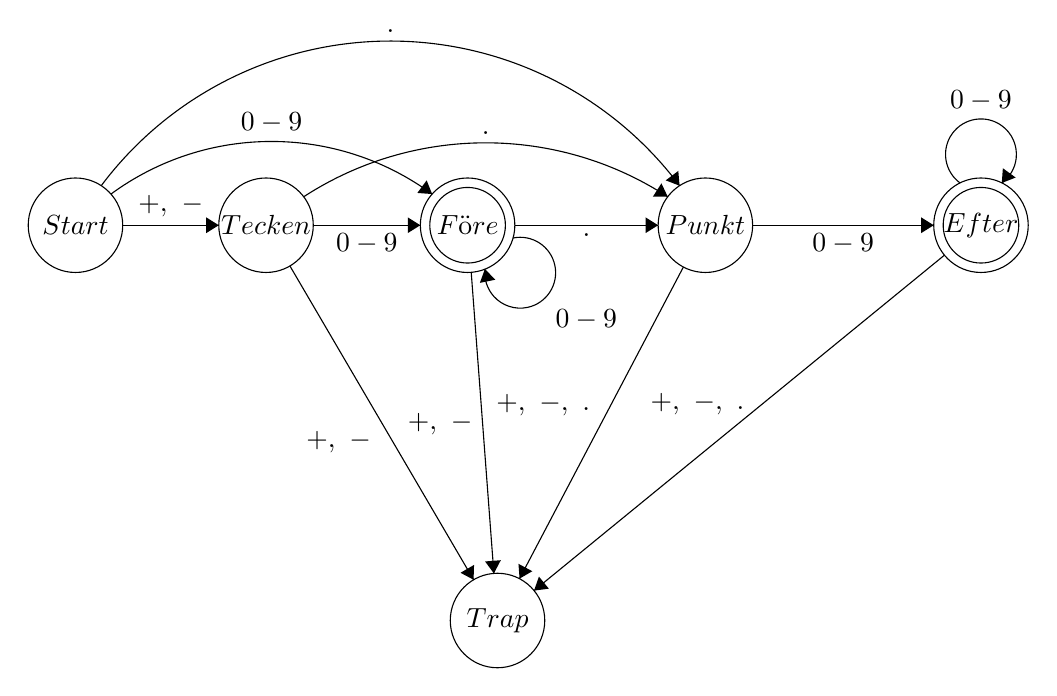
\begin{tikzpicture}[scale=0.2]
\tikzstyle{every node}+=[inner sep=0pt]
\draw [black] (6.1,-29.8) circle (3);
\draw (6.1,-29.8) node {$Start$};
\draw [black] (18.2,-29.8) circle (3);
\draw (18.2,-29.8) node {$Tecken$};
\draw [black] (31,-29.8) circle (3);
\draw (31,-29.8) node {$F\text{ö}re$};
\draw [black] (31,-29.8) circle (2.4);
\draw [black] (46.1,-29.8) circle (3);
\draw (46.1,-29.8) node {$Punkt$};
\draw [black] (63.6,-29.8) circle (3);
\draw (63.6,-29.8) node {$Efter$};
\draw [black] (63.6,-29.8) circle (2.4);
\draw [black] (32.9,-54.9) circle (3);
\draw (32.9,-54.9) node {$Trap$};
\draw [black] (9.1,-29.8) -- (15.2,-29.8);
\fill [black] (15.2,-29.8) -- (14.4,-29.3) -- (14.4,-30.3);
\draw (12.15,-29.3) node [above] {$+,\mbox{ }-$};
\draw [black] (21.2,-29.8) -- (28,-29.8);
\fill [black] (28,-29.8) -- (27.2,-29.3) -- (27.2,-30.3);
\draw (24.6,-30.3) node [below] {$0-9$};
\draw [black] (34,-29.8) -- (43.1,-29.8);
\fill [black] (43.1,-29.8) -- (42.3,-29.3) -- (42.3,-30.3);
\draw (38.55,-30.3) node [below] {$.$};
\draw [black] (49.1,-29.8) -- (60.6,-29.8);
\fill [black] (60.6,-29.8) -- (59.8,-29.3) -- (59.8,-30.3);
\draw (54.85,-30.3) node [below] {$0-9$};
\draw [black] (62.277,-27.12) arc (234:-54:2.25);
\draw (63.6,-22.55) node [above] {$0-9$};
\fill [black] (64.92,-27.12) -- (65.8,-26.77) -- (64.99,-26.18);
\draw [black] (33.875,-30.614) arc (101.92433:-186.07567:2.25);
\draw (36.55,-35.78) node [right] {$0-9$};
\fill [black] (32.1,-32.58) -- (31.78,-33.46) -- (32.76,-33.26);
\draw [black] (7.737,-27.289) arc (143.149:36.851:22.948);
\fill [black] (44.46,-27.29) -- (44.38,-26.35) -- (43.58,-26.95);
\draw (26.1,-17.6) node [above] {$.$};
\draw [black] (20.591,-27.993) arc (123.02792:56.97208:21.207);
\fill [black] (43.71,-27.99) -- (43.31,-27.14) -- (42.77,-27.98);
\draw (32.15,-24.07) node [above] {$.$};
\draw [black] (31.23,-32.79) -- (32.67,-51.91);
\fill [black] (32.67,-51.91) -- (33.11,-51.07) -- (32.11,-51.15);
\draw (31.34,-42.4) node [left] {$+,\mbox{ }-$};
\draw [black] (19.72,-32.39) -- (31.38,-52.31);
\fill [black] (31.38,-52.31) -- (31.41,-51.37) -- (30.55,-51.87);
\draw (24.9,-43.59) node [left] {$+,\mbox{ }-$};
\draw [black] (44.7,-32.46) -- (34.3,-52.24);
\fill [black] (34.3,-52.24) -- (35.11,-51.77) -- (34.23,-51.3);
\draw (38.82,-41.2) node [left] {$+,\mbox{ }-,\mbox{ }.$};
\draw [black] (61.28,-31.7) -- (35.22,-53);
\fill [black] (35.22,-53) -- (36.16,-52.88) -- (35.53,-52.11);
\draw (45.6,-41.86) node [above] {$+,\mbox{ }-,\mbox{ }.$};
\draw [black] (8.351,-27.823) arc (126.30405:53.69595:17.226);
\fill [black] (28.75,-27.82) -- (28.4,-26.95) -- (27.81,-27.75);
\draw (18.55,-23.98) node [above] {$0-9$};
\end{tikzpicture}
\end{center}
% -----------------------------------------------------
% ------------------------ 3 --------------------------
% -----------------------------------------------------
\section{}

Metoden ger följande tabell:
\begin{center}
\begin{tabular}{ |l|l|l| }
\hline
\multicolumn{1}{|c}{$\textbf{state}$}    &  \multicolumn{1}{|c}{$\textbf{0}$}      &  \multicolumn{1}{|c|}{$\textbf{1}$} \\ \hline
$\to \{a, b, c\}$     & $\{b, e\}$        & $\{b, d\}$            \\ \hline
$F\, \{b, e\}$        & $\{a, b, c, d\}$  & $\{d\}$             \\ \hline
$F\, \{b, d\}$        & $\{b, e\}$        & $\{a, b, c, d\}$    \\ \hline
$F\, \{a, b, c, d\}$  & $\{b, e\}$        & $\{a, b, c, d\}$    \\ \hline
$F\, \{d\}$           & $\{e\}$           & $\{a, b, c\}$       \\ \hline
$F\, \{e\}$           & $\{a, b, c\}$     & $\{d\}$             \\ \hline
\end{tabular}
\end{center}

Vilket i sin tur ger denna DFA:
\begin{center}
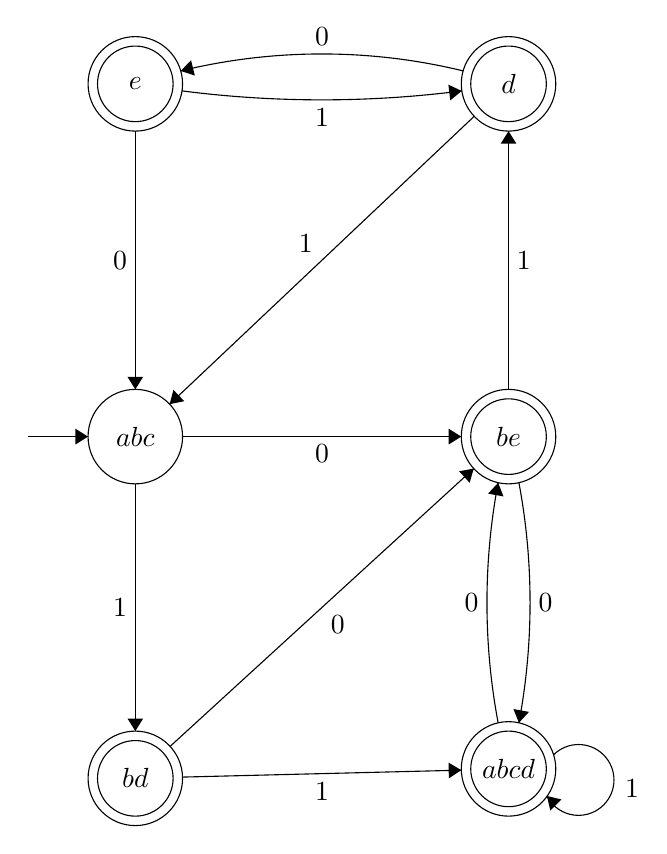
\begin{tikzpicture}[scale=0.2]
\tikzstyle{every node}+=[inner sep=0pt]
\draw [black] (10.7,-33.6) circle (3);
\draw (10.7,-33.6) node {$abc$};
\draw [black] (34.4,-33.6) circle (3);
\draw (34.4,-33.6) node {$be$};
\draw [black] (34.4,-33.6) circle (2.4);
\draw [black] (10.7,-55.3) circle (3);
\draw (10.7,-55.3) node {$bd$};
\draw [black] (10.7,-55.3) circle (2.4);
\draw [black] (34.4,-54.7) circle (3);
\draw (34.4,-54.7) node {$abcd$};
\draw [black] (34.4,-54.7) circle (2.4);
\draw [black] (34.4,-11.2) circle (3);
\draw (34.4,-11.2) node {$d$};
\draw [black] (34.4,-11.2) circle (2.4);
\draw [black] (10.7,-11.2) circle (3);
\draw (10.7,-11.2) node {$e$};
\draw [black] (10.7,-11.2) circle (2.4);
\draw [black] (3.9,-33.6) -- (7.7,-33.6);
\fill [black] (7.7,-33.6) -- (6.9,-33.1) -- (6.9,-34.1);
\draw [black] (13.7,-33.6) -- (31.4,-33.6);
\fill [black] (31.4,-33.6) -- (30.6,-33.1) -- (30.6,-34.1);
\draw (22.55,-34.1) node [below] {$0$};
\draw [black] (10.7,-36.6) -- (10.7,-52.3);
\fill [black] (10.7,-52.3) -- (11.2,-51.5) -- (10.2,-51.5);
\draw (10.2,-44.45) node [left] {$1$};
\draw [black] (35.059,-36.526) arc (10.61134:-10.61134:41.401);
\fill [black] (35.06,-51.77) -- (35.7,-51.08) -- (34.71,-50.9);
\draw (36.27,-44.15) node [right] {$0$};
\draw [black] (34.4,-30.6) -- (34.4,-14.2);
\fill [black] (34.4,-14.2) -- (33.9,-15) -- (34.9,-15);
\draw (34.9,-22.4) node [right] {$1$};
\draw [black] (12.91,-53.27) -- (32.19,-35.63);
\fill [black] (32.19,-35.63) -- (31.26,-35.8) -- (31.93,-36.53);
\draw (23.56,-44.94) node [below] {$0$};
\draw [black] (13.7,-55.22) -- (31.4,-54.78);
\fill [black] (31.4,-54.78) -- (30.59,-54.3) -- (30.61,-55.3);
\draw (22.56,-55.52) node [below] {$1$};
\draw [black] (33.739,-51.774) arc (-169.35842:-190.64158:41.287);
\fill [black] (33.74,-36.53) -- (33.1,-37.22) -- (34.08,-37.4);
\draw (32.53,-44.15) node [left] {$0$};
\draw [black] (37.253,-53.812) arc (135.02737:-152.97263:2.25);
\draw (41.77,-55.96) node [right] {$1$};
\fill [black] (36.84,-56.42) -- (37.05,-57.34) -- (37.76,-56.64);
\draw [black] (13.584,-10.376) arc (103.68256:76.31744:37.905);
\fill [black] (13.58,-10.38) -- (14.48,-10.67) -- (14.24,-9.7);
\draw (22.55,-8.8) node [above] {$0$};
\draw [black] (32.22,-13.26) -- (12.88,-31.54);
\fill [black] (12.88,-31.54) -- (13.81,-31.35) -- (13.12,-30.63);
\draw (21.53,-21.92) node [above] {$1$};
\draw [black] (10.7,-14.2) -- (10.7,-30.6);
\fill [black] (10.7,-30.6) -- (11.2,-29.8) -- (10.2,-29.8);
\draw (10.2,-22.4) node [left] {$0$};
\draw [black] (31.434,-11.647) arc (-82.65902:-97.34098:69.527);
\fill [black] (31.43,-11.65) -- (30.58,-11.25) -- (30.7,-12.25);
\draw (22.55,-12.72) node [below] {$1$};
\end{tikzpicture}
\end{center}

% -----------------------------------------------------
% ------------------------ 4 --------------------------
% -----------------------------------------------------
\section{}
Lägg till en startnod $q_s$ och en slutnod $q_F$ till grafen: 
Börja med att eliminera något state, t.ex. a:
\begin{center}
\begin{tikzpicture}[scale=0.2]
\tikzstyle{every node}+=[inner sep=0pt]
\draw [black] (11.8,-30.5) circle (3);
\draw (11.8,-30.5) node {$q_s$};
\draw [black] (25.2,-30.5) circle (3);
\draw (25.2,-30.5) node {$a$};
\draw [black] (39.2,-23) circle (3);
\draw (39.2,-23) node {$b$};
\draw [black] (39.2,-38.7) circle (3);
\draw (39.2,-38.7) node {$c$};
\draw [black] (54,-30.4) circle (3);
\draw (54,-30.4) node {$d$};
\draw [black] (69,-30.4) circle (3);
\draw (69,-30.4) node {$q_F$};
\draw [black] (69,-30.4) circle (2.4);
\draw [black] (3.3,-30.5) -- (8.8,-30.5);
\fill [black] (8.8,-30.5) -- (8,-30) -- (8,-31);
\draw [black] (14.8,-30.5) -- (22.2,-30.5);
\fill [black] (22.2,-30.5) -- (21.4,-30) -- (21.4,-31);
\draw (18.5,-31) node [below] {$\epsilon$};
\draw [black] (27.84,-29.08) -- (36.56,-24.42);
\fill [black] (36.56,-24.42) -- (35.61,-24.35) -- (36.09,-25.24);
\draw (33.2,-27.25) node [below] {$0$};
\draw [black] (37.877,-20.32) arc (234:-54:2.25);
\draw (39.2,-15.75) node [above] {$0$};
\fill [black] (40.52,-20.32) -- (41.4,-19.97) -- (40.59,-19.38);
\draw [black] (27.79,-32.02) -- (36.61,-37.18);
\fill [black] (36.61,-37.18) -- (36.17,-36.35) -- (35.67,-37.21);
\draw (31.2,-35.1) node [below] {$1$};
\draw [black] (40.523,-41.38) arc (54:-234:2.25);
\draw (39.2,-45.95) node [below] {$1$};
\fill [black] (37.88,-41.38) -- (37,-41.73) -- (37.81,-42.32);
\draw [black] (41.82,-37.23) -- (51.38,-31.87);
\fill [black] (51.38,-31.87) -- (50.44,-31.82) -- (50.93,-32.69);
\draw (47.6,-35.05) node [below] {$0$};
\draw [black] (41.88,-24.34) -- (51.32,-29.06);
\fill [black] (51.32,-29.06) -- (50.82,-28.25) -- (50.38,-29.15);
\draw (45.61,-27.2) node [below] {$1$};
\draw [black] (52.677,-27.72) arc (234:-54:2.25);
\draw (54,-23.15) node [above] {$0\mbox{ }+\mbox{ }1$};
\fill [black] (55.32,-27.72) -- (56.2,-27.37) -- (55.39,-26.78);
\draw [black] (57,-30.4) -- (66,-30.4);
\fill [black] (66,-30.4) -- (65.2,-29.9) -- (65.2,-30.9);
\draw (61.5,-30.9) node [below] {$\epsilon$};
\end{tikzpicture}
\end{center}
\begin{align*}
q_s \to a \to b: & \quad R_1R_2^*R_3+R_4 = \varepsilon\O^*0+\O = 0 \\
q_s \to a \to c: & \quad R_1R_2^*R_3+R_4 = \varepsilon\O^*1+\O = 1
\end{align*}
\begin{center}
\begin{tikzpicture}[scale=0.2]
\tikzstyle{every node}+=[inner sep=0pt]
\draw [black] (39.2,-23) circle (3);
\draw (39.2,-23) node {$b$};
\draw [black] (39.2,-38.7) circle (3);
\draw (39.2,-38.7) node {$c$};
\draw [black] (54,-30.4) circle (3);
\draw (54,-30.4) node {$d$};
\draw [black] (69,-30.4) circle (3);
\draw (69,-30.4) node {$q_F$};
\draw [black] (69,-30.4) circle (2.4);
\draw [black] (26.1,-30.4) circle (3);
\draw (26.1,-30.4) node {$q_s$};
\draw [black] (37.877,-20.32) arc (234:-54:2.25);
\draw (39.2,-15.75) node [above] {$0$};
\fill [black] (40.52,-20.32) -- (41.4,-19.97) -- (40.59,-19.38);
\draw [black] (40.523,-41.38) arc (54:-234:2.25);
\draw (39.2,-45.95) node [below] {$1$};
\fill [black] (37.88,-41.38) -- (37,-41.73) -- (37.81,-42.32);
\draw [black] (41.82,-37.23) -- (51.38,-31.87);
\fill [black] (51.38,-31.87) -- (50.44,-31.82) -- (50.93,-32.69);
\draw (47.6,-35.05) node [below] {$0$};
\draw [black] (41.88,-24.34) -- (51.32,-29.06);
\fill [black] (51.32,-29.06) -- (50.82,-28.25) -- (50.38,-29.15);
\draw (45.61,-27.2) node [below] {$1$};
\draw [black] (52.677,-27.72) arc (234:-54:2.25);
\draw (54,-23.15) node [above] {$0\mbox{ }+\mbox{ }1$};
\fill [black] (55.32,-27.72) -- (56.2,-27.37) -- (55.39,-26.78);
\draw [black] (57,-30.4) -- (66,-30.4);
\fill [black] (66,-30.4) -- (65.2,-29.9) -- (65.2,-30.9);
\draw (61.5,-30.9) node [below] {$\epsilon$};
\draw [black] (28.71,-28.92) -- (36.59,-24.48);
\fill [black] (36.59,-24.48) -- (35.65,-24.43) -- (36.14,-25.3);
\draw (33.65,-27.2) node [below] {$0$};
\draw [black] (28.63,-32.01) -- (36.67,-37.09);
\fill [black] (36.67,-37.09) -- (36.26,-36.24) -- (35.72,-37.09);
\draw (31.65,-35.05) node [below] {$1$};
\draw [black] (17.4,-30.4) -- (23.1,-30.4);
\fill [black] (23.1,-30.4) -- (22.3,-29.9) -- (22.3,-30.9);
\end{tikzpicture}
\end{center}
Forsätt med att ta bort state b:
\begin{align*}
q_s \to b \to d: & \quad R_1R_2^*R_3+R_4 = 00^*1 \\
\end{align*}
\begin{center}
\begin{tikzpicture}[scale=0.2]
\tikzstyle{every node}+=[inner sep=0pt]
\draw [black] (40.1,-38.7) circle (3);
\draw (40.1,-38.7) node {$c$};
\draw [black] (54,-30.4) circle (3);
\draw (54,-30.4) node {$d$};
\draw [black] (69,-30.4) circle (3);
\draw (69,-30.4) node {$q_F$};
\draw [black] (69,-30.4) circle (2.4);
\draw [black] (26.1,-30.4) circle (3);
\draw (26.1,-30.4) node {$q_s$};
\draw [black] (41.423,-41.38) arc (54:-234:2.25);
\draw (40.1,-45.95) node [below] {$1$};
\fill [black] (38.78,-41.38) -- (37.9,-41.73) -- (38.71,-42.32);
\draw [black] (42.68,-37.16) -- (51.42,-31.94);
\fill [black] (51.42,-31.94) -- (50.48,-31.92) -- (50.99,-32.78);
\draw (48.05,-35.05) node [below] {$0$};
\draw [black] (52.677,-27.72) arc (234:-54:2.25);
\draw (54,-23.15) node [above] {$0\mbox{ }+\mbox{ }1$};
\fill [black] (55.32,-27.72) -- (56.2,-27.37) -- (55.39,-26.78);
\draw [black] (57,-30.4) -- (66,-30.4);
\fill [black] (66,-30.4) -- (65.2,-29.9) -- (65.2,-30.9);
\draw (61.5,-30.9) node [below] {$\epsilon$};
\draw [black] (28.68,-31.93) -- (37.52,-37.17);
\fill [black] (37.52,-37.17) -- (37.09,-36.33) -- (36.58,-37.19);
\draw (32.1,-35.05) node [below] {$1$};
\draw [black] (17.4,-30.4) -- (23.1,-30.4);
\fill [black] (23.1,-30.4) -- (22.3,-29.9) -- (22.3,-30.9);
\draw [black] (29.1,-30.4) -- (51,-30.4);
\fill [black] (51,-30.4) -- (50.2,-29.9) -- (50.2,-30.9);
\draw (40.05,-30.9) node [below] {$00^*1$};
\end{tikzpicture}
\end{center}
Ta bort c:
\begin{align*}
q_s \to c \to d: & \quad R_1R_2^*R_3+R_4 = 11^*0 \\
\end{align*}
\begin{center}
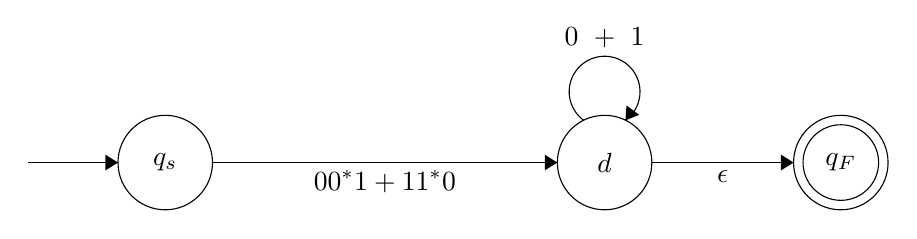
\begin{tikzpicture}[scale=0.2]
\tikzstyle{every node}+=[inner sep=0pt]
\draw [black] (54,-30.4) circle (3);
\draw (54,-30.4) node {$d$};
\draw [black] (69,-30.4) circle (3);
\draw (69,-30.4) node {$q_F$};
\draw [black] (69,-30.4) circle (2.4);
\draw [black] (26.1,-30.4) circle (3);
\draw (26.1,-30.4) node {$q_s$};
\draw [black] (52.677,-27.72) arc (234:-54:2.25);
\draw (54,-23.15) node [above] {$0\mbox{ }+\mbox{ }1$};
\fill [black] (55.32,-27.72) -- (56.2,-27.37) -- (55.39,-26.78);
\draw [black] (57,-30.4) -- (66,-30.4);
\fill [black] (66,-30.4) -- (65.2,-29.9) -- (65.2,-30.9);
\draw (61.5,-30.9) node [below] {$\epsilon$};
\draw [black] (17.4,-30.4) -- (23.1,-30.4);
\fill [black] (23.1,-30.4) -- (22.3,-29.9) -- (22.3,-30.9);
\draw [black] (29.1,-30.4) -- (51,-30.4);
\fill [black] (51,-30.4) -- (50.2,-29.9) -- (50.2,-30.9);
\draw (40.05,-30.9) node [below] {$00^*1+11^*0$};
\end{tikzpicture}
\end{center}
Sist ta bort d:
\begin{align*}
q_s \to d \to q_F: & \quad R_1R_2^*R_3+R_4 = (00^*1+11^*0)(0+1)^* \\
\end{align*}
\begin{center}
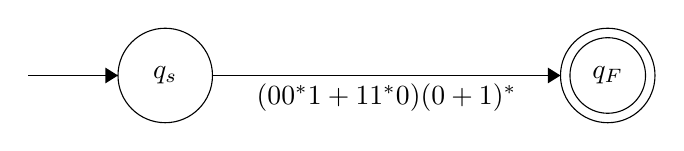
\begin{tikzpicture}[scale=0.2]
\tikzstyle{every node}+=[inner sep=0pt]
\draw [black] (54.2,-30.4) circle (3);
\draw (54.2,-30.4) node {$q_F$};
\draw [black] (54.2,-30.4) circle (2.4);
\draw [black] (26.1,-30.4) circle (3);
\draw (26.1,-30.4) node {$q_s$};
\draw [black] (17.4,-30.4) -- (23.1,-30.4);
\fill [black] (23.1,-30.4) -- (22.3,-29.9) -- (22.3,-30.9);
\draw [black] (29.1,-30.4) -- (51.2,-30.4);
\fill [black] (51.2,-30.4) -- (50.4,-29.9) -- (50.4,-30.9);
\draw (40.15,-30.9) node [below] {$(00^*1+11^*0)(0+1)^*$};
\end{tikzpicture}
\end{center}

\textbf{Svar: } $(00^*1+11^*0)(0+1)^*$

% -----------------------------------------------------
% ------------------------ 5 --------------------------
% -----------------------------------------------------
\section{}

Vi börjar med att markera alla par av tillstånd där ena är accept och den andra är reject:

\begin{center}
\begin{tabular}{|*{6}{c|}}
                             \cline{1-1}
  \textbf{a}              \\ \cline{1-2}
  0 & \textbf{b}          \\ \cline{1-3}
  0 &  & \textbf{c}       \\ \cline{1-4}
  0 &  &  & \textbf{d}    \\ \cline{1-5}
  0 &  &  &  & \textbf{e} \\ \cline{1-5}
\end{tabular}
\end{center}

Första iterationen:
\begin{align*}
    \{b, c\} : \{\delta(b, 0), \delta(c, 0)\} &= \{a, e\} \text{ är markerad, markera } \{b, c\} \\
    \{b, d\} : \{\delta(b, 0), \delta(d, 0)\} &= \{a, e\} \text{ är markerad, markera } \{b, d\} \\
    \{b, e\} : \{\delta(b, 0), \delta(e, 0)\} &= \{a\} \text{ är inte markerad, kolla 1} \\
    \{b, e\} : \{\delta(b, 1), \delta(e, 1)\} &= \{d\} \text{ är inte markerad, markera inte} \\
    \{c, d\} : \{\delta(c, 0), \delta(d, 0)\} &= \{e\} \text{ är inte markerad, kolla 1} \\
    \{c, d\} : \{\delta(c, 1), \delta(d, 1)\} &= \{a\} \text{ är inte markerad, markera inte} \\
    \{c, e\} : \{\delta(c, 0), \delta(e, 0)\} &= \{a, d\} \text{ är markerad, så markera } \{c, e\} \\
    \{d, e\} : \{\delta(d, 0), \delta(e, 0)\} &= \{a, e\} \text{ är markerad, så markera } \{d, e\} \\
\end{align*}
\begin{center}
\begin{tabular}{|*{6}{c|}}
                             \cline{1-1}
  \textbf{a}              \\ \cline{1-2}
  0 & \textbf{b}          \\ \cline{1-3}
  0 & 1 & \textbf{c}       \\ \cline{1-4}
  0 & 1 &  & \textbf{d}    \\ \cline{1-5}
  0 &   & 1 & 1 & \textbf{e} \\ \cline{1-5}
\end{tabular}
\end{center}

Andra iterationen:
\begin{align*}
    \{b, e\} : \{\delta(b, 0), \delta(e, 0)\} &= \{a\} \text{ är inte markerad, kolla 1} \\
    \{b, e\} : \{\delta(b, 1), \delta(e, 1)\} &= \{d\} \text{ är inte markerad, markera inte} \\
    \{c, d\} : \{\delta(c, 0), \delta(d, 0)\} &= \{e\} \text{ är inte markerad, kolla 1} \\
    \{c, d\} : \{\delta(c, 1), \delta(d, 1)\} &= \{a\} \text{ är inte markerad, markera inte} \\
\end{align*}
\begin{center}
\begin{tabular}{|*{6}{c|}}
                             \cline{1-1}
  \textbf{a}              \\ \cline{1-2}
  0 & \textbf{b}          \\ \cline{1-3}
  0 & 1 & \textbf{c}       \\ \cline{1-4}
  0 & 1 &  & \textbf{d}    \\ \cline{1-5}
  0 &   & 1 & 1 & \textbf{e} \\ \cline{1-5}
\end{tabular}
\end{center}

Inga ändringar skedde i andra iterationen vilket betyder att vi är färdiga. Vi får att $b \approx e$ och $c \approx d$. Den minimala DFA blir då:
\begin{center}
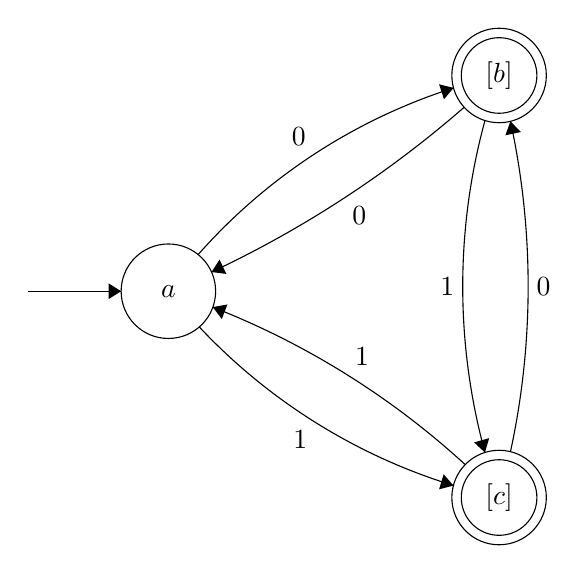
\begin{tikzpicture}[scale=0.2]
\tikzstyle{every node}+=[inner sep=0pt]
\draw [black] (18.8,-30.8) circle (3);
\draw (18.8,-30.8) node {$a$};
\draw [black] (39.8,-17.1) circle (3);
\draw (39.8,-17.1) node {$[b]$};
\draw [black] (39.8,-17.1) circle (2.4);
\draw [black] (39.8,-43.9) circle (3);
\draw (39.8,-43.9) node {$[c]$};
\draw [black] (39.8,-43.9) circle (2.4);
\draw [black] (9.9,-30.8) -- (15.8,-30.8);
\fill [black] (15.8,-30.8) -- (15,-30.3) -- (15,-31.3);
\draw [black] (20.691,-28.472) arc (138.54589:107.69344:36.395);
\fill [black] (36.91,-17.89) -- (35.99,-17.66) -- (36.3,-18.61);
\draw (27.08,-21.59) node [above] {$0$};
\draw [black] (36.9,-43.135) arc (-107.08711:-136.82551:37.061);
\fill [black] (36.9,-43.14) -- (36.28,-42.42) -- (35.99,-43.38);
\draw (27.17,-39.65) node [below] {$1$};
\draw [black] (37.582,-19.119) arc (-48.92734:-64.83333:69.208);
\fill [black] (21.54,-29.58) -- (22.48,-29.7) -- (22.05,-28.79);
\draw (30.93,-25.41) node [below] {$0$};
\draw [black] (21.623,-31.813) arc (68.59659:47.49079:51.565);
\fill [black] (21.62,-31.81) -- (22.19,-32.57) -- (22.55,-31.64);
\draw (31.1,-35.57) node [above] {$1$};
\draw [black] (38.902,-41.038) arc (-164.72891:-195.27109:40.011);
\fill [black] (38.9,-41.04) -- (39.17,-40.13) -- (38.21,-40.4);
\draw (36.99,-30.5) node [left] {$1$};
\draw [black] (40.523,-20.011) arc (12.21842:-12.21842:49.561);
\fill [black] (40.52,-20.01) -- (40.2,-20.9) -- (41.18,-20.69);
\draw (42.15,-30.5) node [right] {$0$};
\end{tikzpicture}
\end{center}

% -----------------------------------------------------
% ------------------------ 6 --------------------------
% -----------------------------------------------------
\section{}
\begin{enumerate}[label=(\alph*)]
    \item 
Här kan vi skapa en automat som räknar hur många a:s man har i x-led och hur många b:s man har i y-led. Skulle det någonsin hända att $\#a(w) \le \#b(w)$ så går vi till ett trap-tillstånd.
\begin{center}
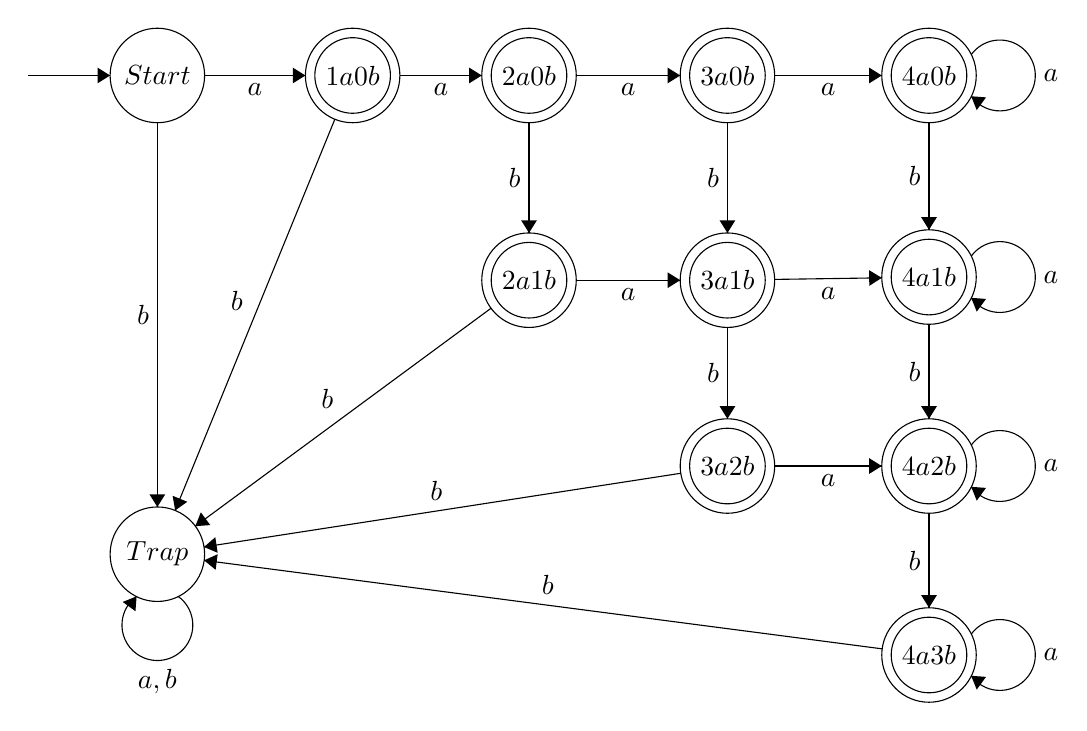
\begin{tikzpicture}[scale=0.2]
\tikzstyle{every node}+=[inner sep=0pt]
\draw [black] (12.2,-16.7) circle (3);
\draw (12.2,-16.7) node {$Start$};
\draw [black] (24.6,-16.7) circle (3);
\draw (24.6,-16.7) node {$1a0b$};
\draw [black] (24.6,-16.7) circle (2.4);
\draw [black] (35.8,-16.7) circle (3);
\draw (35.8,-16.7) node {$2a0b$};
\draw [black] (35.8,-16.7) circle (2.4);
\draw [black] (48.4,-16.7) circle (3);
\draw (48.4,-16.7) node {$3a0b$};
\draw [black] (48.4,-16.7) circle (2.4);
\draw [black] (35.8,-29.7) circle (3);
\draw (35.8,-29.7) node {$2a1b$};
\draw [black] (35.8,-29.7) circle (2.4);
\draw [black] (48.4,-29.7) circle (3);
\draw (48.4,-29.7) node {$3a1b$};
\draw [black] (48.4,-29.7) circle (2.4);
\draw [black] (12.2,-47.1) circle (3);
\draw (12.2,-47.1) node {$Trap$};
\draw [black] (48.4,-41.5) circle (3);
\draw (48.4,-41.5) node {$3a2b$};
\draw [black] (48.4,-41.5) circle (2.4);
\draw [black] (61.2,-16.7) circle (3);
\draw (61.2,-16.7) node {$4a0b$};
\draw [black] (61.2,-16.7) circle (2.4);
\draw [black] (61.2,-29.5) circle (3);
\draw (61.2,-29.5) node {$4a1b$};
\draw [black] (61.2,-29.5) circle (2.4);
\draw [black] (61.2,-41.5) circle (3);
\draw (61.2,-41.5) node {$4a2b$};
\draw [black] (61.2,-41.5) circle (2.4);
\draw [black] (61.2,-53.5) circle (3);
\draw (61.2,-53.5) node {$4a3b$};
\draw [black] (61.2,-53.5) circle (2.4);
\draw [black] (4,-16.7) -- (9.2,-16.7);
\fill [black] (9.2,-16.7) -- (8.4,-16.2) -- (8.4,-17.2);
\draw [black] (15.2,-16.7) -- (21.6,-16.7);
\fill [black] (21.6,-16.7) -- (20.8,-16.2) -- (20.8,-17.2);
\draw (18.4,-17.2) node [below] {$a$};
\draw [black] (27.6,-16.7) -- (32.8,-16.7);
\fill [black] (32.8,-16.7) -- (32,-16.2) -- (32,-17.2);
\draw (30.2,-17.2) node [below] {$a$};
\draw [black] (38.8,-16.7) -- (45.4,-16.7);
\fill [black] (45.4,-16.7) -- (44.6,-16.2) -- (44.6,-17.2);
\draw (42.1,-17.2) node [below] {$a$};
\draw [black] (13.523,-49.78) arc (54:-234:2.25);
\draw (12.2,-54.35) node [below] {$a,b$};
\fill [black] (10.88,-49.78) -- (10,-50.13) -- (10.81,-50.72);
\draw [black] (35.8,-19.7) -- (35.8,-26.7);
\fill [black] (35.8,-26.7) -- (36.3,-25.9) -- (35.3,-25.9);
\draw (35.3,-23.2) node [left] {$b$};
\draw [black] (48.4,-19.7) -- (48.4,-26.7);
\fill [black] (48.4,-26.7) -- (48.9,-25.9) -- (47.9,-25.9);
\draw (47.9,-23.2) node [left] {$b$};
\draw [black] (12.2,-19.7) -- (12.2,-44.1);
\fill [black] (12.2,-44.1) -- (12.7,-43.3) -- (11.7,-43.3);
\draw (11.7,-31.9) node [left] {$b$};
\draw [black] (48.4,-32.7) -- (48.4,-38.5);
\fill [black] (48.4,-38.5) -- (48.9,-37.7) -- (47.9,-37.7);
\draw (47.9,-35.6) node [left] {$b$};
\draw [black] (33.39,-31.48) -- (14.61,-45.32);
\fill [black] (14.61,-45.32) -- (15.56,-45.25) -- (14.96,-44.44);
\draw (23,-37.9) node [above] {$b$};
\draw [black] (38.8,-29.7) -- (45.4,-29.7);
\fill [black] (45.4,-29.7) -- (44.6,-29.2) -- (44.6,-30.2);
\draw (42.1,-30.2) node [below] {$a$};
\draw [black] (51.4,-16.7) -- (58.2,-16.7);
\fill [black] (58.2,-16.7) -- (57.4,-16.2) -- (57.4,-17.2);
\draw (54.8,-17.2) node [below] {$a$};
\draw [black] (51.4,-29.65) -- (58.2,-29.55);
\fill [black] (58.2,-29.55) -- (57.39,-29.06) -- (57.41,-30.06);
\draw (54.8,-30.11) node [below] {$a$};
\draw [black] (61.2,-19.7) -- (61.2,-26.5);
\fill [black] (61.2,-26.5) -- (61.7,-25.7) -- (60.7,-25.7);
\draw (60.7,-23.1) node [left] {$b$};
\draw [black] (61.2,-32.5) -- (61.2,-38.5);
\fill [black] (61.2,-38.5) -- (61.7,-37.7) -- (60.7,-37.7);
\draw (60.7,-35.5) node [left] {$b$};
\draw [black] (51.4,-41.5) -- (58.2,-41.5);
\fill [black] (58.2,-41.5) -- (57.4,-41) -- (57.4,-42);
\draw (54.8,-42) node [below] {$a$};
\draw [black] (45.44,-41.96) -- (15.16,-46.64);
\fill [black] (15.16,-46.64) -- (16.03,-47.01) -- (15.88,-46.02);
\draw (29.91,-43.71) node [above] {$b$};
\draw [black] (63.88,-15.377) arc (144:-144:2.25);
\draw (68.45,-16.7) node [right] {$a$};
\fill [black] (63.88,-18.02) -- (64.23,-18.9) -- (64.82,-18.09);
\draw [black] (63.88,-28.177) arc (144:-144:2.25);
\draw (68.45,-29.5) node [right] {$a$};
\fill [black] (63.88,-30.82) -- (64.23,-31.7) -- (64.82,-30.89);
\draw [black] (63.88,-40.177) arc (144:-144:2.25);
\draw (68.45,-41.5) node [right] {$a$};
\fill [black] (63.88,-42.82) -- (64.23,-43.7) -- (64.82,-42.89);
\draw [black] (61.2,-44.5) -- (61.2,-50.5);
\fill [black] (61.2,-50.5) -- (61.7,-49.7) -- (60.7,-49.7);
\draw (60.7,-47.5) node [left] {$b$};
\draw [black] (63.88,-52.177) arc (144:-144:2.25);
\draw (68.45,-53.5) node [right] {$a$};
\fill [black] (63.88,-54.82) -- (64.23,-55.7) -- (64.82,-54.89);
\draw [black] (58.23,-53.11) -- (15.17,-47.49);
\fill [black] (15.17,-47.49) -- (15.9,-48.09) -- (16.03,-47.1);
\draw (37,-49.71) node [above] {$b$};
\draw [black] (23.47,-19.48) -- (13.33,-44.32);
\fill [black] (13.33,-44.32) -- (14.1,-43.77) -- (13.17,-43.39);
\draw (17.66,-31) node [left] {$b$};
\end{tikzpicture}
\end{center}

\newpage
\item
Välj $s = a^{p+5}\,b^{p+4}$

$s \in L_2$ då det uppfyller det första kravet (dock inte det andra). Vi kan nu välja $x, y$ och $z$ så att $s=xyz$ enligt:
\begin{flalign*}
& x = a^k, \quad k > 0 \\
& y = a^m, \quad m > 0, \quad k+m \le p \\
& z = a^{p-m-k+5}\,\, b^{p+4} 
\end{flalign*}
Vi kan nu pumpa y neråt:
$$xy^0z = a^k a^{p-m-k+5} \, b^{p+4} = a^{p-m+5}\, b^{p+4}$$
%Alltså får vi: 
%$$s = xyz = a^k a^m a^{p-m-k+5} \, b^{p+4} = a^{p+5}\, b^{p+4}$$

Men nu ser vi att mängden a:s är mindre än eller lika med mängden b:s då:
$$p-m+5 \le p + 4$$
alltså tillhör inte denna strängen $L_2$, vilket leder till att pumplemmat inte håller och att $L_2$ inte är reguljärt.
\end{enumerate}

% -----------------------------------------------------
% ------------------------ 7 --------------------------
% -----------------------------------------------------
\section{}

\begin{enumerate}[label=(\alph*)]
    \item 
Välj $s$ så att $s \in T$ och att $|s| = 2^p$. Vi kan nu välja $x, y$ och $z$ så att $s=xyz$ enligt:
\begin{flalign*}
& |x] = k, \quad k > 0 \\
& |y| = 1, \quad k + 1 \le p \\
& |z| = 2^p-k-1
\end{flalign*}
%Vi får: 
%$$|s| = |xyz| = |k + m + 2^p - k - m| = 2^p$$

Om vi nu pumpar y uppåt får vi:
$$|xy^2z| = k + 2 + 2^p - 1 - k = 2^p - 1$$
vilket uppenbart har udda längd och alltså inte tillhör $T$, och då leder till att $T$ inte är reguljärt enligt pumplemmat.

    \item 
Definiera $\equiv_T$ så att:
$$x \equiv_T y \text{ omm för varje } z \in \Sigma^* (xz \in T \iff yz \in T)$$

%$x \equiv_T y \text{ omm för varje } z \in \{0, 1\}^* \text{ så är } |xz| = 2^a \iff |yz| = 2^b \text{ där } a,b \in \mathbb{N}$


Sedan gör vi ett motsägelsebevis. Antag att:
$$x \equiv_T y \text{ där } |x|=2^i \text{ och } |y|=2^k, \quad i \ne k, \quad i, k \in \mathbb{N}$$

Välj $z=\bar{x}$, alltså att $|z|=2^i$. Då får vi att: 
$$xz \in T \text{ då } xz = x\bar{x} \text{ och }|xz| = 2^{i+1}$$
Dock så är:
$$yz \notin T \text{ då } |yz| = 2^k + 2^i \ne 2^{k+1} \text{ då } k \ne i$$
Det är alltså omöjligt för $yz$ att vara ett Thue-Morse-tal då det längden inte kan skrivas som en enda 2-potens.

Vi skulle alltså behöva en unik ekvivalensklass för varje $i$, vilket innebär ett oändligt antal klasser, alltså kan inte T vara reguljär. 
\end{enumerate}

\end{document}
